\chapter*{Annexes}
\addcontentsline{toc}{chapter}{Annexes}

\section*{Annexe 1 : Remise à 0 du code}
\addcontentsline{toc}{section}{Annexe 1 : Remise à 0 du code}
\label{ANNEXE1}
Cette annexe est utile si jamais vous avez téléchargé le code au travers de la commande : 

\begin{lstlisting} [style=MyBashStyle]
	git clone https://github.com/Kymaro/DrancIoT.git
\end{lstlisting}\\

Si jamais vous avez fait des modifications du code et que vous êtes dans l'incapacité de revenir en arrière sur votre \textit{RaspberryPi}. Si vous êtes encore dans l'éditeur de fichier, fermer le terminal pour vous déconnecter de la \textit{RaspberryPi}. Connectez vous à nouveau en \textit{SSH} sur votre station et effectuer les étapes :\\

\begin{lstlisting} [style=MyBashStyle]

	cd
	cd DrancIoT/
	git reset --hard
\end{lstlisting}\\

Les fichiers devraient alors revenir à leur état initial comme si vous veniez de le télécharger. Vous pouvez alors recommencer la sous-partie~\ref{CONFIG} page~\pageref{CONFIG} \textbf{sans recommencer la commande :}\\

\begin{lstlisting}[style=MyBashStyle]
	sudo pip install azure-servicebus
\end{lstlisting}\\


\section*{Annexe 2 : Alimentation PoE de la \textit{RaspberryPi}}
\addcontentsline{toc}{section}{Annexe 2 : Alimentation PoE de la \textit{RaspberryPi}}\\

L'une des conditions du cahier des charges était que la station soit alimenté en PoE. PoE est l'anagramme de "Power over Ethernet". Comprenez en français "Alimentation électrique par câble Ethernet". Il faut savoir qu'en plus d'assurer le transfert de données, un câble réseaux peut, par cette technologie, alimenter des périphériques.\\

Le câble délivre alors une tension de 48V pour une puissance maximal d'environ 13 Watts. 

	Cela signifie que votre station sera alimenté non pas par une prise secteur classique, mais bel et bien par son câble ethernet au travers de sa prise RJ45 de la \textit{RaspberryPi}. Malheureusement cette dernière ne gère pas la technologie PoE. Elle ne peut donc pas convertir l'alimentation 48V qu'elle recevrait en alimentation 5V dont elle a besoin. C'est pour cette raison que vous allez utiliser un \textit{PoE Splitter}.
	
	\begin{figure}[H]
	\begin{center}
		\makebox[\textwidth]{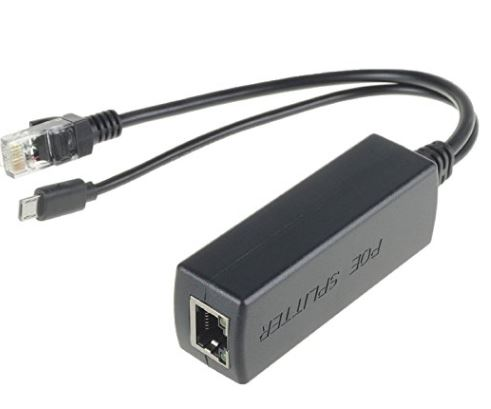
\includegraphics[width=.6\paperwidth]{images/PoE.jpg}}
	\end{center}
		\caption{ \textit{PoE Splitter}}
	\end{figure}\\
	
Ce petit adaptateur vous permettra, comme vous pouvez le voir, de séparer l'alimentation PoE et les données dans un connecteur respectivement micro USB et RJ45. De cette façon, nous pouvons alimenter notre station en \textit{PoE}.